\chapter{Lorem ipsum dolor sit amet}

É importante apresentar, ao início de cada capítulo, uma breve introdução sobre o mesmo. Essa introdução, não deve conter mais do que 2 parágrafos. Uma sugestão, é relembrar de forma sucinta o que foi apresentado no capítulo anterior, e relacionar com o conteúdo deste capítulo.

Também é aconselhável, que cada capítulo possua uma sessão de conclusão. A importância desta é discutida adiante. Esta recomendações não são uma regra do IFC, mas têm sido bastante utilizadas no BSI. 

\section{Figuras e legendas}\label{sec:figs}

Essa sessão apresenta como utilizar figuras e tabelas ao longo do TCC. Também é apresentado o uso das legendas para esses dois tipos de recursos. 

Temos dois exemplos, a figura~\ref{fig:exemploFig1} e a figura~\ref{fig:exemploFig2}.

\begin{figure}[htbp]
\centering
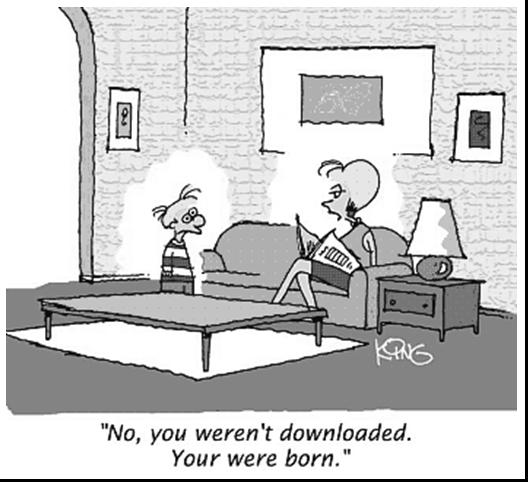
\includegraphics[width=.5\textwidth]{Figuras/fig1.jpg}
\caption{Uma figura típica}
\label{fig:exemploFig1}
\end{figure}

\begin{figure}[htbp]
\centering
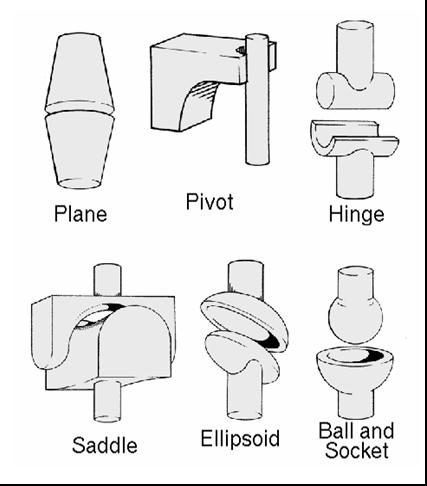
\includegraphics[width=.3\textwidth]{Figuras/fig2.jpg}
\caption{Essa figura é um exemplo de figura contendo uma legenda utilizando mais do que uma única linha.}
\label{fig:exemploFig2}
\end{figure}

A figura~\ref{fig:exemplo_png} que é um exemplo de figura no formato PNG. Além desse formato, também pode-se utilizar figuras no formato JPG e GIF. Figuras no formato EPS também podem ser utilizadas, porém a geração do PDF final não pode ser feita utilizando diretamente o comando \texttt{pdflatex}.

\begin{figure}[htbp]
\centering

\includegraphics[width=.5\textwidth]{Figuras/latex-logo.png}
\caption{Essa figura é um exemplo de figura no formato PNG.}
\label{fig:exemplo_png}
\end{figure}

Podemos utilizar tabelas também (tabela~\ref{tab:exTabela}). Nesse caso tente evitar o uso de fundos com cores ou sombras, e evite linhas de grade grossas, duplas ou desnecessárias. A legenda da tabela deve ser colocada sempre antes dela, no topo.

\begin{table}[htbp]
\centering
\caption{Um exemplo de tabela}
\label{tab:exTabela}
\begin{tabular}{l|c|r} \hline
Cabeçalho Esquerda & Cabeçalho Centro & Cabeçalho Direita \\ 
\hline \hline
Linha 1 Coluna 1   & Linha 1 Coluna 2 & Linha 1 Coluna 3  \\
Linha 2            & Coluna do meio   & Coluna 3          \\
Coluna 1           & Linha 3          & Última célula     \\
\hline
\end{tabular}
\end{table}

\section{Códigos-fontes de linguagens de programação}

Uma linguagem de programação é um método padronizado para expressar instruções para um computador. É um conjunto de regras sintáticas e semânticas usadas para definir um programa de computador. Uma linguagem permite que um programador especifique precisamente sobre quais dados um computador vai atuar, como estes dados serão armazenados ou transmitidos e quais ações devem ser tomadas sob várias circunstâncias.

Depois que inventaram o computador , perceberam que ele não servia prá nada. Durante milhares de anos o computador ficou relegado a segundo plano e apenas calculadoras eram usadas! Mas um tecelão francês chamado Jacquard criou o primeiro programa para suas máquinas de tecer. Com inveja, Blaise Pascal, inventou a linguagem Pascal para jovens com retardamento mental. Naquela época os computadores ainda eram muito rudimentares e não foi possível utilizar de forma satisfatória todos os recursos das Linguagens de Programação. Muito tempo depois Charles Babbage criou a máquina Diferencial prá fazer subtrações e a máquina Somatorial para fazer somas. Como dava um trabalho muito duro construir máquinas para cada uma das operações, ele pediu à sua assistente Lady Ada Lovelace prá resolver o problema. Ada então criou a Linguagem de Programação Ada, muito utilizada na Guerra do Golfo pelos Militares Americanos.

\subsection{Python}

Python é uma linguagem de programação de alto-nível interpretada, interativa, orientada a objetos, de tipagem dinâmica e forte. A linguagem foi projetada com a filosofia de enfatizar a importância do esforço do programador sobre o esforço computacional. Prioriza a legibilidade do código sobre a velocidade ou expresividade. Combina uma sintaxe concisa e clara com os recursos poderosos de sua biblioteca padrão e por módulos e frameworks desenvolvidos por terceiros. O código \ref{mediapy} é um exemplo de código-fonte em Python.

%\begin{figure}[htbp] 
\lstinputlisting[language=python,caption={Cálculo da média entre dois números escrito na linguagem Python},label=mediapy]{Codigos/media.py}
%\centering
%\caption{Cálculo da média entre dois números escrito na linguagem Python}
%\label{fig:mediapy}\end{figure}

Python é a principal sucessora de Logo, porém é também uma calculadora de linha de comando, orientada à identação. Costuma ser o destino preferencial dos programadores Ruby, quando estes finalmente se dão conta que estão usando um ``Perl 2.0''. 

\subsection{C++}

O C++ é uma linguagem de programação de alto nível com facilidades para o uso em baixo nível, multiparadigma e de uso geral. Desde os anos 1990 é uma das linguagens comerciais mais populares, sendo bastante usada também na academia por seu grande desempenho e base de utilizadores.  O código \ref{mediacpp} é um exemplo de código-fonte em C++.

%\begin{figure}[htbp]
\lstinputlisting[language=C++, caption={Cálculo da média entre dois números escrito na linguagem C++}, label=mediacpp]{Codigos/media.cpp}
%\centering
%\caption{Cálculo da média entre dois números escrito na linguagem C++}
%\label{fig:mediacpp}
%\end{figure}

C++ é uma linguagem de programação, muitas vezes é referida como Cpp , criada por Steve Ballmer com o propósito de deixar programador loucos, em um plano para eliminar a concorrência da Microsoft (que usa a programação orientada a gambiarras em seus programas).

Suas principais características são o paradigma orientado à desorientação e falta de sentido em geral, a incoerência de sintaxe, e ser melhor do que Java. A linguagem incorpora todas as vantagens da linguagem C, isto é, nenhuma, e todos os benefícios da orientação a objetos, isto é, poder fazer uma classe Quadrado que herda da classe Retângulo, com um incrivel custo em performance por isso. 

\subsection{Java}

Java é uma linguagem de programação orientada a objeto desenvolvida na década de 90 pelo programador James Gosling, na empresa Sun Microsystems. Diferentemente das linguagens convencionais, que são compiladas para código nativo, a linguagem Java é compilada para um ``bytecode'' que é executado por uma máquina virtual. A linguagem de programação Java é a linguagem convencional da Plataforma Java, mas não sua única linguagem.  O código \ref{mediajava} é um exemplo de código-fonte em Java.

%\begin{figure}[htbp]
\lstinputlisting[language=java, caption={Cálculo da média entre dois números escrito na linguagem Java}, label=mediajava]{Codigos/media.java}
%\caption{Cálculo da média entre dois números escrito na linguagem Java}
%\label{fig:mediajava}
%\end{figure}

A Linguagem Java é famosa por ser muito eficiente. A maioria dos programas mais complexos é escrita em Java, como o Adobe Photoshop ou o Microsoft Windows ME, podendo funcionar com apenas 640 bytes de RAM, e atingir velocidades instantâneas. Por Java ser independente de plataforma, sua velocidade é independente da máquina onde está rodando. Por padrão, Java 1.2 pode calcular um loop infinito em menos de 1.2 minutos, daí vem esse número na linguagem. A palavra ``Java'' vem de um dialeto da Indonésia que quer dizer ``Espetáculo do crescimento'', o que explica programas com poucos KBytes no disco possuírem dezenas de MBytes na memória principal.

\subsection{Listas numeradas e de itens}

Se quisermos uma lista numerada, devemos fazer assim:

\begin{enumerate}
\item este é o primeiro item;
\item este é o segundo item;
\item e este é o terceiro e último item.
\end{enumerate}

Por outro lado, uma lista de itens é feita desse modo:

\begin{itemize}
\item este é o primeiro item;
\item este é o segundo item;
\item e este é o terceiro e último item.
\end{itemize}

\section{Referências}

Referências bibliográficas precisam ser não ambíguas e uniformes. Recomendamosdar os nomes dos autores entre espaços, por exemplo \cite{knuth:84},
\cite{boulic:91}, e \cite{smith:99}. Em caso de dúvidas, consulte o manual de metodologia para desenvolvimento do TCC, disponível na página do IFC ou na página do BSI.

Citações longas com mais de três linhas devem seguir ao seguinte formato:

\begin{citacao}
O IPSEC foi concebido como uma extensão de terceira camada ao TCP/IP, ou seja estende o próprio protocolo IP. Na verdade, para o IPv6; depois o IPSEC também foi portado para o IPv4.
A idéia original do IPSEC é permitir a comunicação segura e *transparente* entre quaisquer dois nós da Internet, desde que os dois implementem IPSEC. Se os dois têm IPSEC, automaticamente há troca de chaves e criptografia. Esse modo de funcionamento do IPSEC denomina-se ``modo transporte''~\cite{epx}. 
\end{citacao}

% ---
\section{Aliquam vestibulum fringilla lorem}
% ---

\lipsum[1]

\lipsum[2-3]
